%# -*- coding: utf-8 -*-
%%采用 xelatex + ctex 文档类
\documentclass[fancyhdr,fntef,UTF8,oneside,12pt,a4paper, winfonts]{ctexbook}
%%%%%!!!请将您的个人信息按照注释正确填写!!!%%%%%

%%%%%封面及摘要内容,中文 
\newcommand{\department} {计算机科学与技术系}  	%院系
\newcommand{\major}      {计算机科学与技术} 	%专业方向
\newcommand{\thesistitle}{关系数据库模式与本体间的语义映射发现方法初探} 	%论文题目
\newcommand{\grade}      {2008级}	    %年级
\newcommand{\NJUID}      {081221043}%学号
\newcommand{\myname}     {贾存鑫}		%姓名
\newcommand{\advisor}    {胡伟}		%指导老师姓名
\newcommand{\advisorjob} {讲师}		%指导老师职称
\newcommand{\enteryear}  {2008}		%入学年份

%%%%%封面及摘要内容,英文
\newcommand{\edepartment} {Department of Computer Science and Technology}	%院系
\newcommand{\emajor}      {Computer Science and Technology}				%专业方向
\newcommand{\ethesistitle}{A Pilot Study on Discovering Semantic Mappings Between Relational Database Schemas and OWL Ontologies}			%论文题目
\newcommand{\emyname}     {Cunxin Jia}			%姓名
\newcommand{\eadvisor}    {Wei Hu}				%指导老师姓名

%% 字体设置
\setCJKfamilyfont{song}{NSimSun}
\setCJKfamilyfont{zhongsong}{STZhongsong}
\setCJKfamilyfont{kai}{KaiTi}
\setCJKfamilyfont{hei}{SimHei}
\setCJKfamilyfont{fs}{FangSong} %FangSong_GB2312
\setCJKfamilyfont{li}{LiSu}
\setCJKfamilyfont{yy}{YouYuan}
\newcommand{\song}{\CJKfamily{song}}
\newcommand{\zs}{\CJKfamily{zhongsong}}
\newcommand{\kai}{\CJKfamily{kai}}
\newcommand{\hei}{\CJKfamily{hei}}
\newcommand{\fs}{\CJKfamily{fs}}
\newcommand{\li}{\CJKfamily{li}}
\newcommand{\yy}{\CJKfamily{yy}}
\setmainfont{Times New Roman} %英文字体使用Times New Roman
%\setmainfont[SmallCapsFont=LMRomanCaps10]{Times New Roman}
%Times New Roman 字体不包括 Small Caps 形状,如果要使用,需设定 Small Caps 字体,如 LMRomanCaps10

\renewcommand{\ULthickness}{0.7pt}
\newcommand{\myuline}[2]      {\uline{\makebox[#1]{#2}}}
\newcommand{\NJUTunderline}[1]{\uline{\hfill{#1}\hfill}}
\footnotesep=10pt

\usepackage{amsmath,amsfonts,amssymb}
\usepackage{array}
\usepackage{booktabs,multirow,colortbl,longtable}
\usepackage{verbatim}
\usepackage{lipsum}
\usepackage{comment}
\usepackage{footnpag}
\usepackage{amsthm} %Added by Cunxin Jia
\usepackage{algorithm} %Added by Cunxin Jia
\usepackage{algorithmic} %Added by Cunxin Jia


%% 加载图形宏包
\usepackage{graphicx}
%% 设置图片目录
\graphicspath{{figures/}}
\usepackage[config]{subfig}
\usepackage{indentfirst}
\usepackage[neverdecrease]{paralist}
\let\itemize\compactitem
\let\enditemize\endcompactitem
\let\enumerate\compactenum
\let\endenumerate\endcompactenum
\let\description\compactdesc
\let\enddescription\endcompactdesc

%%设置浮动体(表格、图片)标题格式
\DeclareCaptionLabelFormat{nju}{{\zihao{5}\song #1~#2}}
\DeclareCaptionLabelSeparator{nju}{\hspace{1em}}
\DeclareCaptionFont{nju}{\zihao{5}\song}
\captionsetup{labelformat=nju,labelsep=nju,font=nju}
\captionsetup[table]{position=top,belowskip={12bp-\intextsep},aboveskip=6bp}
\captionsetup[figure]{position=bottom,belowskip={12bp-\intextsep},aboveskip=6bp}

%% 超链接、目录
\usepackage{hyperref}
\usepackage{xcolor}
\definecolor{darkblue}{rgb}{0,0,0.55}
\hypersetup{CJKbookmarks,bookmarksnumbered,%
			colorlinks,unicode=true,%
			linkcolor=black,%
			citecolor=darkblue,%
			plainpages=false,%
			bookmarksopen=true,%
			bookmarksopenlevel=1,
			pdfstartview=FitH,
			pdftitle={\thesistitle},
    		pdfauthor={\myname},
    		pdfcreator={XeLaTeX with NJUThesis template designed by pkuphy},}
\usepackage{tabularx}%只要把tabularx包的引用放到hyperref包之后,正文脚注编号就能正常生成超链接。
%%版面控制
\usepackage{geometry}
\geometry{top=3.5cm,bottom=3.5cm,left=3.2cm,right=3.2cm}
%\geometry{headheight=2.6cm,headsep=5mm,footskip=13mm}
\parskip 0.5ex plus 0.25ex minus 0.25ex

\renewcommand{\textfraction}{0.15}
\renewcommand{\topfraction}{0.85}
\renewcommand{\bottomfraction}{0.65}
\renewcommand{\floatpagefraction}{0.60}


\fancypagestyle{myfancy}{%
\fancyhf{}
\fancyhead[C]{\small \song\leftmark}
\fancyfoot[C]{\small \thepage}
\renewcommand{\headrulewidth}{0.7pt}
}
\pagestyle{myfancy}


\setcounter{secnumdepth}{3}%%自动编号到 subsubsection

\CTEXsetup[nameformat={\hei\zihao{-2}}]{chapter}
\CTEXsetup[titleformat={\hei\zihao{-2}}]{chapter}
\CTEXsetup[beforeskip={-20pt}]{chapter}
\CTEXsetup[afterskip={20pt}]{chapter}
\CTEXsetup[format={\hei\zihao{-3}}]{section}
\CTEXsetup[nameformat={\bf\hei\zihao{-3}}]{section}
\CTEXsetup[beforeskip={-3ex plus -1ex minus -.2ex}]{section}
\CTEXsetup[afterskip={1.0ex plus .2ex}]{section}
\CTEXsetup[format={\hei\zihao{-4}}]{subsection}
\CTEXsetup[nameformat={\bf\hei\zihao{-4}}]{subsection}
\CTEXsetup[beforeskip={-2.5ex plus -1ex minus -.2ex}]{subsection}
\CTEXsetup[afterskip={1.0ex plus .2ex}]{subsection}
\CTEXoptions[contentsname={目\qquad 录}]
\CTEXoptions[listfigurename={插\qquad 图}]
\CTEXoptions[listtablename={表\qquad 格}]

%% 中文破折号,来自清华模板
\newcommand{\pozhehao}{\kern0.3ex\rule[0.8ex]{2em}{0.1ex}\kern0.3ex}

\newenvironment{abstract}{
\thispagestyle{plain}
\pagenumbering{Roman}
\pdfbookmark[0]{中文摘要}{abstract}
\begin{center}
{\bf\kai\zihao{-2} \uuline{南~京~大~学~本~科~生~毕~业~论~文~中~文~摘~要}}
\end{center}
\bigskip

\noindent
\begin{minipage}{\textwidth}
\kai\zihao{4}%
\noindent{毕业论文题目:}\NJUTunderline{\thesistitle}\\
\NJUTunderline{\department}{院系}\NJUTunderline{\major}{专业}
\NJUTunderline{\enteryear}{级本科生}\hfill\\{姓名:}\NJUTunderline{\myname}\\
{指导教师(姓名、职称):}\uline{\hfill\advisor 、\advisorjob\hfill}
\end{minipage}

\vskip 1cm
\begin{center}
{\heiti\zihao{-3} 摘\quad 要}
\end{center}\par
\kai\zihao{-4}
}{}
\newcommand\keywords[1]{\vspace{2ex}\noindent{\hei 关键词:} {\kai #1}}

\newenvironment{englishabstract}{
\clearpage
\thispagestyle{plain}
\pdfbookmark[0]{英文摘要}{englishabstract}
\begin{center}
{\bf\kai\zihao{-2} \uuline{南~京~大~学~本~科~生~毕~业~论~文~英~文~摘~要}}
\end{center}
\bigskip

\noindent
{\zihao{4}%
%\begin{description}
%\item{THESIS:} {\bf\ethesistitle}
%\item{DEPARTMENT:} {\bf\edepartment}
%\item{SPECIALIZATION:} {\bf\emajor}
%\item{UNDERGRADUATE:} {\bf\emyname}
%\item{MENTOR:} {\bf\eadvisor}
%\end{description}
THESIS: {\bf\ethesistitle} \\
DEPARTMENT: {\bf\edepartment} \\
SPECIALIZATION: {\bf\emajor} \\
UNDERGRADUATE: {\bf\emyname} \\
MENTOR: {\bf\eadvisor} \\
}
\vskip 1cm
%\begin{description}
\noindent{\zihao{4} ABSTRACT:}
%\end{description}
}{}

\newcommand\englishkeywords[1]{\vspace{2ex}\noindent{\zihao{4}KEYWORDS:} #1}

\renewcommand\maketitle{%
\clearpage
\thispagestyle{empty}
\pdfbookmark[0]{封面}{cover}

\begin{center}
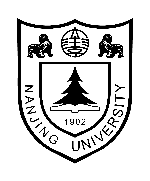
\includegraphics[width=1.96cm]{logo} \\
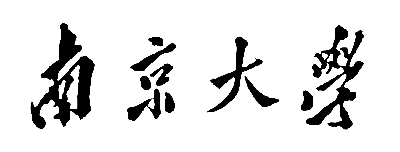
\includegraphics[height=2cm]{name} \\
\vskip 1cm
\zs
\zihao{0} 本~~科~~毕~~业~~论~~文\\
\vskip 2in\zihao{3}
\begin{minipage}{0.9\textwidth}
院\qquad 系\NJUTunderline{\department}\\[3mm]
专\qquad 业\NJUTunderline{\major}\\[3mm]
题\qquad 目{\normalsize\NJUTunderline{\thesistitle}}\\[3mm]
年\qquad 级\myuline{4.5cm}{\grade}{\hfill}学\qquad 号\myuline{4cm}{\NJUID}\\[3mm]
学生姓名\NJUTunderline{\myname}\\[3mm]
指导老师\myuline{4.5cm}{\advisor}{\hfill}职\qquad 称\myuline{4cm}{\advisorjob}\\[3mm]
论文提交日期\NJUTunderline{2012年5月27日}
\end{minipage}
\end{center}
\clearpage
\thispagestyle{empty}
\vspace*{\stretch{1}}
{\kai\zihao{-3}
\noindent
\begin{tabular}{ccr}
\begin{CJKfilltwosides}{3.5cm}学号\end{CJKfilltwosides} & : & \makebox[6cm][r]{\NJUID}\\
\begin{CJKfilltwosides}{3.5cm}论文答辩日期\end{CJKfilltwosides} & : & 2012年5月28日\\
\begin{CJKfilltwosides}{3.5cm}指导教师\end{CJKfilltwosides} & : & \uline{\qquad\qquad\quad}(签字)\\
\end{tabular}
}
}

\newcommand\makeenglishtitle{%
\clearpage
\thispagestyle{empty}
\begin{center}
\vspace*{20pt}
\bf\zihao{2} \ethesistitle
\vskip \stretch{1}
\normalfont\zihao{4} by
\vskip 3pt
\bf\zihao{4} \emyname
\vskip \stretch{1}
\normalfont\zihao{4} Directed by
\vskip 3pt
\bf\zihao{4} \eadvisor
\vskip \stretch{2}
\normalfont\large \edepartment \\Nanjing University
\vskip 30pt
\CTEXoptions[today=old]
\normalfont\large May 27,2012
\vskip 20pt
\it\large Submitted in full fulfilment of the requirements\\for the degree of Bachelor of Science in Computer Science.
\end{center}
}


\begin{document}
\maketitle
\makeenglishtitle
\frontmatter
\normalfont
\begin{abstract}
伴随语义网的发展,语义网本体数量激增。然而万维网上绝大多数的数据仍存储在关系数据
库中。建立关系数据库模式与语义网本体间的映射是一种实现两者之间互操作性的有效途径
。本文提出一种基于语义的关系数据库模式与OWL本体间的映射方法SMap,包含简单映射发
现和复杂映射学习两个阶段。在简单映射发现阶段,首先通过逆向工程规则将关系数据库模
式和本体中的元素对应地分入不同类别,再为每个元素构建虚拟文档并计算它们之间的相似
度,其中针对不同类别的元素设计了不同的虚拟文档抽取方案。在复杂映射学习阶段,基于
已发现的简单映射以及重叠的数据库记录和本体实例,自动化地生成训练事实数据,然后运
用归纳逻辑编程算法学习出多种类型的基于Horn规则的复杂映射。使用AJAX技术和JAVA编程
语言设计并实现了一个原型系统,真实数据集上的实验结果表明,SMap在简单映射发现和复
杂映射学习上均明显优于现有的关系数据库模式与本体间映
射方法。
\end{abstract}

\keywords{本体映射; 模式匹配; 关系数据库; 虚拟文档; 归纳逻辑编程}

\begin{englishabstract}
Ontologies proliferate with the development of the Semantic Web. Most data on 
the Web, however, are still stored in relational databases (RDBs). Createing
mappings between RDB schemas and ontologies is an effective way for
establishing the interoperability between them. In this paper, we propose SMap
-- a semantic approach to create mappings between RDB schemas and OWL ontologies.
SMap consists of two main stages: finding simple mappings and learning complex
mappings. In the first stage, the elements in an RDB schema and an ontology are
classified correspondingly into different categories, and the virtual documents
for the elements are built in terms of their categories and then matched for
similarities. In the second stage, based upon the pre-found simple mappings as
well as overlapped RDB records and ontology instances, the facts for inductive
logic programming are automatically collected, in order to learn different types
of Horn-rule-like complex mappings. We designed and implemented a prototype 
system using AJAX and JAVA. Experimental results on real-world datasets
demonstrate that, SMap outperforms existing approaches significantly on both
simple mapping finding and complex mapping learning. 
\end{englishabstract}

\englishkeywords{ontology mapping; schema matching; relational database;
virtual document; inductive logic programming}
\clearpage

\pdfbookmark[0]{目录}{tableofcontents}
\tableofcontents
\listoffigures
\listoftables  %这条命令是表格目录,需要的话可以启用;上面那条是图片目录,不需要可以注释掉或者直接删除

\mainmatter
\zihao{-4}
\song
\chapter{引言}
\label{chap00}
语义Web(Semantic Web)是Web(万维网)的一个重要发展方向,它提供一个通用框架,
使得数据的共享和重用可以跨越应用系统、企业和社区的边界。在原始Web上只有文档的
交换和共享,语义Web以RDF(Resource Description Framework)为基础,而RDF以URI
(Uniform Resource Identifier)作为标识机制、XML作为语法,能够将各种不同应用中
的数据和服务容易地集成起来。本体(ontology)在语义Web中扮演着重要的角色,语义
Web本体一般是指使用RDFS(RDF Schema)或者OWL(Web Ontology Language)等语言描述
的本体,其中定义了类(class)、属性(property)和实例(instance)。而类、属性和
实例又可统称为实体(entity)。近年来,有关RDF数据查询的SPARQL和有关规则表示的
RIF(Rule Interchange Format)等技术也日趋成熟,标志着语义Web的数据模型、本体
语言、规则语言和数据存储等技术基础已经奠定。

随着语义网(Semantic Web)的快速发展,语义网数据大幅增长。本体(ontology)作为
语义网的基础,它是领域知识概念化和模型化的一种重要途径,被用来描述数据的
语义信息。迄今为止,语义网搜索引擎Falcons\cite{1}已经采集到超过2.5万个语义网本
体。尽管语义网技术在生命科学等领域已经取得了阶段性成功,但是它距离广泛应用仍有
很长一段距离,其中一个主要的原因是由于当前万维网上绝大多数的数据是以关系数据库
的方式存储(约占77.3\%,俗称``deep Web''\cite{2}),导致语义网应用不能自由地访
问和操纵这些数据,从而限制了语义网的发展。万维网的发明人和语义网的倡导者Tim
Berners-Lee先生也撰文指出,世界上的很多数据仍然封闭在数据库中,尚未在万维网上
以资源的形式公开发布\cite{3}。

关系数据库和本体的数据互操作性问题,一部分可归结为关系数据库模式和本体间的映射
问题\cite{4}。传统关系数据库中,关系表的结构及其完整性约束都由关系数据库
模式定义,并且关系数据库模式和本体间存在着许多近似的对应关系。例如关系数据库
模式中的列可以对应到本体中的属性。事实上,关系数据库中的许多原语都属于一阶逻辑
范畴\cite{5},而最常见的OWL DL本体\cite{6}的逻辑基础为描述逻辑语言
$\mathcal{SHOIN(D)}$,描述逻辑是一阶逻辑的一个子集。因此,建立关系数据库模式和
本体间的映射在理论上是可行的。

现实世界中,不同的关系数据库通常拥有不同的数据模式,而万维网和语义网的分布性
使得不同领域乃至相同领域的不同组织也可能定义不同的本体,这造成了现实中存在众多
异构的关系数据库模式和本体。由于数量、规模等原因,通过人工方式发现关系数据库模式
和本体间的映射非常耗时耗力。国内外研究人员已经提出了一些(半)自动化的关系数据
库模式和本体间的映射方法\cite{4,7}。这些方法大致可分为两类:一类是发现关系数据
库模式中元素(表、列)和本体中元素(类、属性)之间一对一的简单映射;另一类是基于
简单映射生成多对多的复杂映射。

本文提出一种基于语义的关系数据库模式和本体间的映射方法SMap,既能够发现元素之间的
简单映射也能学习复杂映射,具体流程见图\ref{fig:0}。SMap首先采用逆向工程规则,启
发式地将关系数据库模式和本体中的元素对应地划分到4个不同类别中,再针对不同类别中
的元素引入不同的相邻元素的自然语言描述来构建虚拟文档,通过计算虚拟文档间的相似
度来发现元素之间的简单映射。接下来,基于这些简单映射以及重叠的实例数据(数据库
记录、本体实例)生成训练事实集合,采用一种自底向上的归纳逻辑编程算法GOLEM
\cite{8}学习出元素之间的3种复杂映射。这些以Horn规则形式表达的复杂映射可以很容易
地转换为条件查询。在6组真实数据集上的实验结果表明,SMap无论是在简单映射发现还是
在复杂映射学习上均明显优于5个现有的关系数据库模式和本体间的映射方法。

\begin{figure}[htdp]
\centerline{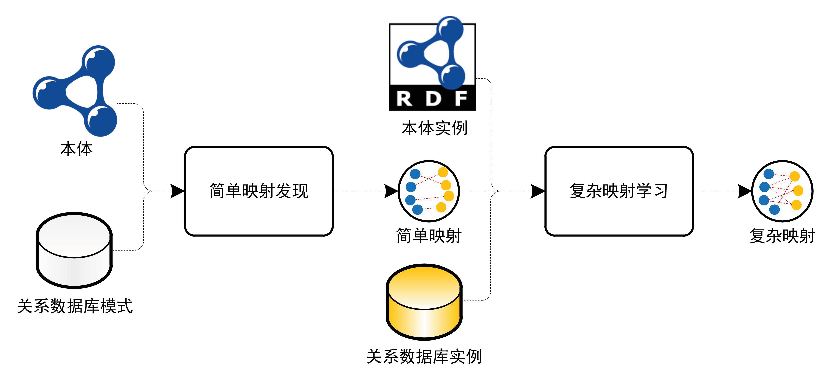
\includegraphics{0.eps}}
\caption{关系数据库模式和本体间语义映射发现流程}
\label{fig:0}
\end{figure}

文章的组织结构如下:第\ref{chap01}章介绍相关工作并给出问题定义;第\ref{chap02}、
\ref{chap03}章分别介绍简单映射的发现方法和复杂映射的学习方法;第\ref{chap04}章
介绍原型系统的设计实现并测试方法的有效性;最后总结全文。

\chapter{关系数据库模式与本体间映射的问题描述}
\label{chap01}

\section{相关工作}

现有工作从多个方面研究了关系数据库模式和本体间的映射问题,例如设计映射系统的框架
、提出具体映射算法以及定义映射结果的语法语义。有关介绍请参见研究综述\cite{4,7}。
根据是否给定本体,现有工作可分为如下两类:

\begin{itemize}
	\item 从已有关系数据库模式中采用信息抽取的方法生成新的本体
	\item 发现已有关系数据库和给定本体之间的关联
\end{itemize}

第一类工作主要针对本体不存在的情况,如Relational.OWL\cite{33}可将关系数据库自动翻
译为OWL Full本体,将关系数据库模式中的关系和属性分别表示为元类Table和Column的实例
,将关系数据库中元组表示为代表模式的类的实例。类似工作DataMaster\cite{34}和ROSEX
\cite{35}在Relational.OWL的基础上进行了扩充。D2RQ\cite{11}利用了逆向工程的方法和
一些预先定义的规则,可将关系数据库模式自动化地翻译为RDFS本体,并且允许用户参与修
正映射结果。文献\cite{13}定义了一组Datalog的规则,可将关系数据库模式及其实例数据
直接映射为新的本体,并且证明这种直接映射具有信息保持、查询保持以及单调性的性质,
而后又针对语义保持的性质提出两种改进直接映射,最终得到单调性和语义保持不能共存的
结论。

第二类工作针对给定本体的情况,如DartGrid是一个中医药领域的数据集成系统\cite{25},
其中的DartMapping模块提供了一个可视化的工具,帮助领域专家手工定义关系数据库模式与
本体间的映射。OntoMat-Reverse\cite{26}使用逆向工程规则和基于编辑距离的文本相似度
计算方法,半自动地发现关系数据库中表/列和本体中类/属性间的映射,与它类似的工作还
有RONTO\cite{27}、Marson\cite{24}等。OntoGrate框架\cite{28}首先将每个关系数据库模
式转化为对应的DB本体,然后借助记录链接和多关系数据挖掘等技术,高度自动化地发现DB
本体和其他语义网本体之间的映射。此外OntoGrate还设计了一种称为Web-PDDL的映射语言,
将针对本体的查询转换为SQL查询。类似地,StdTrip\cite{29}也是将关系数据库模式转化
为本体后再实施本体映射。MapOnto\cite{10}使用树状结构作为数据库模式和本体的中间转
换模型,基于预先发现的简单映射,在两个中间模型上迭代地传播这些映射,最终发现关系
数据库模式中元素和本体元素之间的多对多映射,并以Horn字句的形式表达。Marson则基于
具有分类特性的关系数据库列(例如性别的取值有``男''和``女''),运用决策数算法构造
一类具有包含关系的复杂映射,可以转化为基于视图的查询。

对比上述研究工作,在简单映射发现方面,本文提出了基于虚拟文档的方法,通过考察元素周
围的各种邻居元素的自然语言描述,显著提高了映射结果的效果。在复杂映射学习方面,除
MapOnto和Marson以外,其它工作还很少考虑复杂映射。MapOnto仅利用属性的定义域/值域
的兼容性构建一种句法层次上的复杂映射,Marson则是基于具有分类特性的列构造一类包含
查询,而本文运用归纳逻辑编程算法,能够从重叠实例数据中学习出多种复杂映射,覆盖面更
广。另外,数据库领域中的模式映射\cite{30}和语义网领域中的本体映射\cite{31}已经有
不少有借鉴意义的相关研究,也有工作试图将数据库模式转换为本体后再寻找映射
\cite{28,29},但是由于关系数据库模式和本体之间不存在完美的兼容关系,所以这种转换
通常是不完备的,造成了后续本体映射的精度损失。


\section{问题描述}

数据模型是在概念层面对数据进行的描述和定义,隐藏了许多低层次的存储细节\cite{9}。
对某一类数据的结构、联系和约束的描述称为数据模式。关系数据库和本体基于两种不同的
数据模型,本文主要研究这两种异构数据模型之间的映射发现。

关系数据库模式是一个关系模式的有限集合。一个关系模式由关系名、关系中的属性名及其
关联的定义域组成。关系模式中的定义域包含定义域名和一个取值的集合。关系数据库模式
中的完整性约束定义了施加在数据上的语义约束。本文用$R$表示一个关系(relation),
$A$表示一个属性 (attribute)。$type(A)$表示$A$的定义域名,$rel(A)$表示$A$所属的
关系。$pk(R)$表示R中的主键,$ref(A)$表示$A$引用的属性。


本体是对某一概念模型的显式规范说明。如果没有特别说明,文章所涉及的本体是指使用
OWL语言\cite{6}描述的语义网本体。使用$C$表示一个本体类(class),$P$表示一个属性
(property)。$P_d$表示一个数据类型属性(data type property),$P_o$表示一个对象
属性(object property)。$d(P)$表示$P$的定义域,$r(P)$表示其值域。

在信息数据集成、数据仓库中的数据集成等研究中,Horn子句常被用于表达关系数据
源和以描述逻辑表示的概念模型之间的联系\cite{10}。一个Horn子句是一组文字
(literal)的析取,其中文字是应用到常量或变量上的谓词。能够被满足的(与事实相符
的)文字被称作正文字,否则是负文字。一个子句被称为Horn子句当且仅当它最多有一个正
文字。Horn规则是一种Horn子句,仅包含一个正文字和至少一个负文字,可以表示成
$H \mbox{:-} L_1 \wedge L_2 \wedge \ldots \wedge L_k $的形式,其中$H$称为规则头
或者后继,$L_1 \wedge L_2 \wedge \ldots \wedge L_k$称为规则体或者前驱。本文基于
Horn规则来定义关系数据库模式与本体间的语义映射。

\newtheorem{defn}{\heiti{定义}}
\begin{defn}[关系数据库模式与本体间映射]
一个关系数据库模式$\mathcal{S}$和一个本体$\mathcal{O}$之间的映射发现一个语义映射
集合$\mathcal{M}=\{m_1,\ldots,m_n\}$。每个$m_i(1 \le i\le n)$表示成一个Horn规则
的形式:$T(\overrightarrow{X}) \mbox{\rm:-} \varPhi (\overrightarrow{X},
\overrightarrow{Y}) $,其中$T(\overrightarrow{X})$
表示$\mathcal{S}$中的一个关系R的单个|R|元谓词文字,|R|为R中属性的数量;而
$\varPhi (\overrightarrow{X},\overrightarrow{Y})$是由$\mathcal{O}$中表示类的一
元谓词文字和表示属性的二元谓词文字构成的合取式。
\end{defn}

请注意,本文研究假设目标本体和关系数据库模式均已独立存在,而以D2RQ\cite{11}和
文献\cite{12,13}为代表的工作则是针对本体不存在的情况,考虑如何将关系数据库模式
转换为新本体,与本文工作有本质区别。

\section{关系数据库模式和本体实例}
为方便理解,以下给出一个关系数据库模式和一个本体的例子。

图\ref{fig:onto}为一个本体,包含了4个类:
\emph{Course}、\emph{Student}、\emph{Undergraduate}和\emph{Graduate}, 其中
\emph{Undergraduate}和\emph{Graduate}是\emph{Student}的子类;6个属性:
\emph{takesCourse}、\emph{taOf}、\emph{hasSID}、\emph{hasStudentName}、
\emph{hasCID}和\emph{hasCourseName},其中前两个属性为对象属性,其余为数据类型
属性。


\begin{figure}[htbp]
\centerline{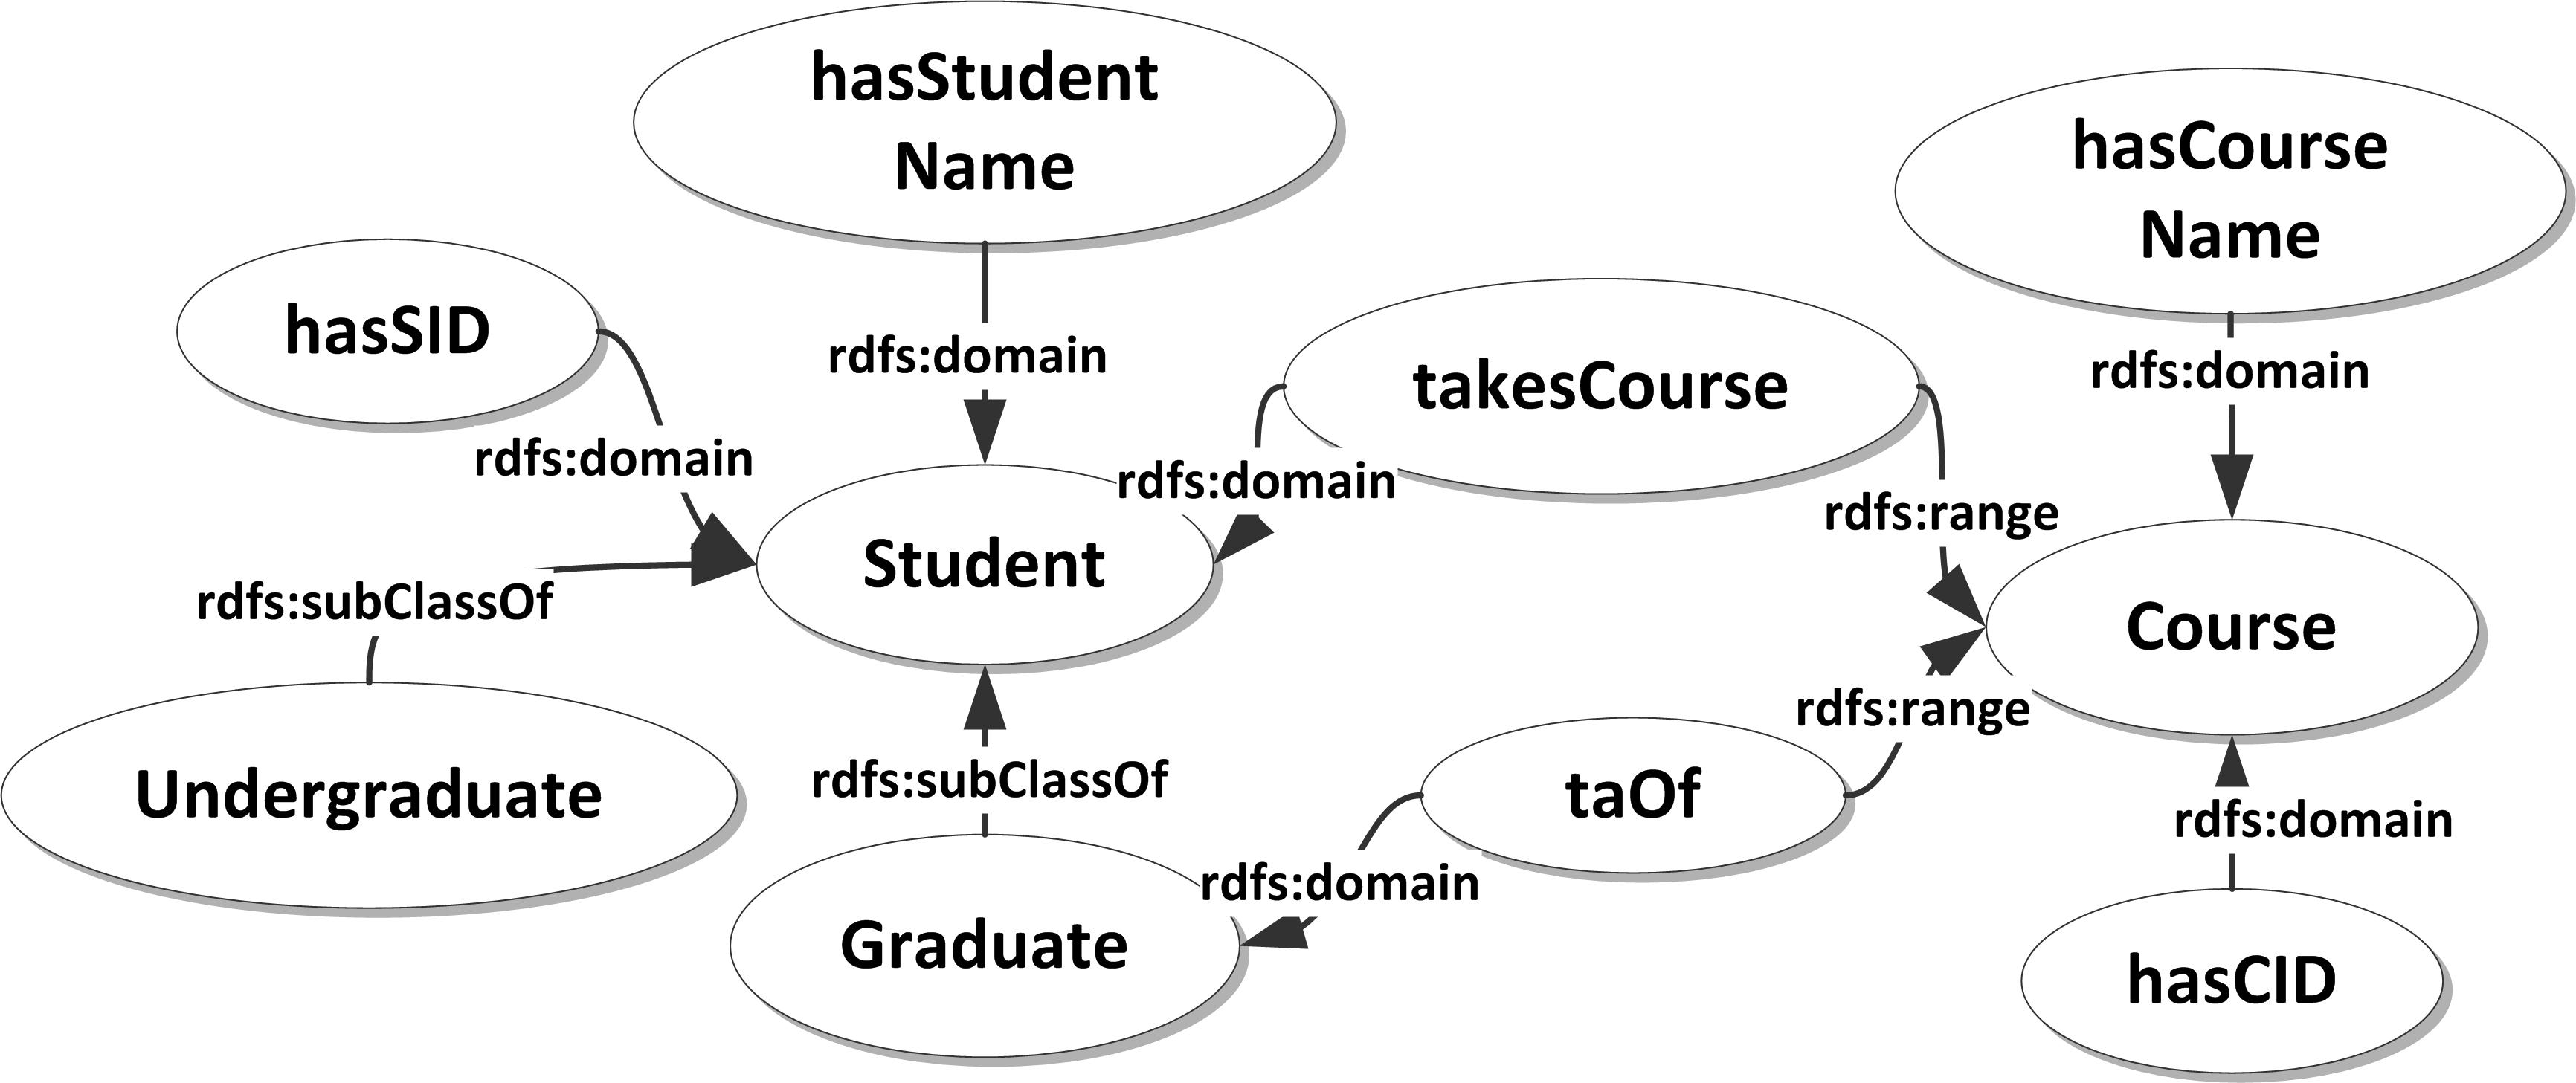
\includegraphics{ontology}}
\caption{本体示例}
\label{fig:onto}
\end{figure}

图\ref{fig:db}为一个关系数据库模式,包含3个关系:\emph{student}、\emph{course}
和\emph{takes\_course};带下划线的属性为关系的主键,比如\emph{student}中的
\emph{\underline{sid}};箭头表示引用完整性约束,例如\emph{takes\_course}中外
键\emph{\underline{cid}}引用了\emph{course}中的\emph{\underline{cid}}。

\begin{figure}[htbp]
\centerline{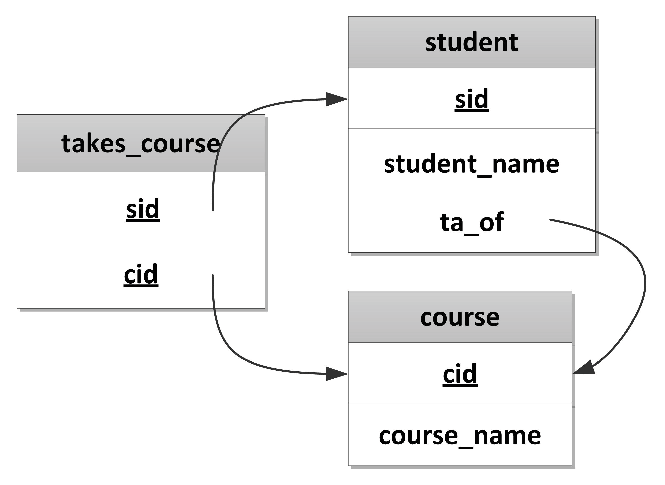
\includegraphics[height=5cm]{DB}}
\caption{关系数据库模式示例}
\label{fig:db}
\end{figure}


构建图\ref{fig:db}中关系数据库模式和图\ref{fig:onto}中本体间的映射,既可以发
现简单映射,如
$\mathcal{S}$:\emph{Course.course\_name}和$\mathcal{O}$:\emph{hasCourseName};
也可以发现复杂映射,如$\mathcal{S}$:\emph{student}(\emph{sid,\_,\_}) 
:- $\mathcal{O}$:\emph{Student}(\emph{A}),
 $\mathcal{O}$:\emph{hasSID}(\emph{A,sid})。



\chapter{简单映射的发现}
\label{chap02}

简单映射的发现主要分为两个步骤:基于逆向工程规则的元素分类和基于虚拟文档的简单
映射发现。

\section{元素类型分类}
\label{2:1}
文献\cite{14}在对关系数据库逆向工程的研究中,将关系分为4种不相交的类型:强实体
类型关系(strong entity relation,简称SER)、弱实体类型关系(weak entity
relation,简称WER)、常规关系类型关系(regular relationship relation,简称RRR)
、以及特殊关系类型关系(specific relationship relation,简称SRR)。而属性也可
简单地分为两类:外键类型属性(FKA)和非外键类型属性(NFKA)。

具体判别规则如下:如果一个关系的所有主键均不是外键,则该关系属于强实体类型关系
,例如图\ref{fig:db}中的\emph{student};如果关系的所有主键均为外键,并且主键数目
大于2,则属于常规关系类型关系,例如图\ref{fig:db}中的\emph{takes\_courese};
而对于弱实体类型关系和特殊关系类型关系,则需要推理和人工参与。如果一个关系是强
实体类型关系的子关系,也就是说该关系中的部分主键作为外键,并且仅只想某一个强实
体类型关系,则这个关系属于弱实体类型关系;对于特殊关系类型关系的判断与之相似。
如果上述自动推理不能判断,则需要人工参与识别。另外,有时还需要存储的实例数据加
以验证。对于外键类型属性和非外键类型属性的判别则相对简单,在此不再赘述。

一般而言,一个实体类型关系可以映射到本体中的一个类,而一个关系类型关系可以映射
到本体中的一个对象属性。例如,图\ref{fig:db}所示的关系\emph{student}可以与类
\emph{Student}映射;而关系\emph{takes\_course}可以与对象属性\emph{takesCourse}
映射。类似地,如果一个属性是外键类型属性,则它可以映射到本体中的一个对象属性,
而一个非外键属性则既可以映射到本体中的一个数据类型属性,也可以映射到一个对象属
性。这里需要注意一种例外情况,如果一个关系是关系类型关系,则它所有的作为主键
并且同时作为外键的属性不需要参与映射过程,如图\ref{fig:db}中的关系
\emph{takes\_course}的属性\emph{\underline{sid}}和\emph{\underline{cid}}
不必包含在映射结果中,否则会导致重复。

根据上述启发式规则,本文把关系数据库模式和本体中的元素对应地划分为4类:

\begin{itemize}
\item{$\{\{SER\} \cup \{WER\} \} \times \{C\}$}
\item{$\{\{RRR\} \cup \{SRR\} \} \times \{P_o\}$}
\item{$\{FKA\} \times \{P_o\}$}
\item{$\{NFKA\} \times \{\{P_o\} \cup \{P_d\}\}$}
\end{itemize}

此外,还设计一些预处理步骤来协调关系数据模式和本体的不同特性。首先,一个关系类
型关系允许映射到本体中的两个具有互反关系(owl:inverseOf)的对象属性。其次
,关系数据库模式中的多元关系($\ge3$)应被具体化(reify)为多个二元关系,因为OWL
本体只能表达一元或二元关系。另外,还对关系数据库和本体中常见的数据类型做抽象,
将主要数据类型归为整型、浮点型、字符型、日期型和布尔型。请注意,这里的预处理步
骤并不是完备的,但是它们涵盖了较多的实际情况。

\section{基于虚拟文档的简单映射发现}
\label{2:2}
受文献\cite{15}的启发,本文考虑引入关系数据库模式和本体间的结构特征来体现它们对
应的语义信息。比如关系数据库中的引用完整性约束连接了两个关系,而OWL本体可以表示
为RDF图的形式,该图结构包含了重要的语义信息。

本文为关系数据库模式和本体中的每个元素构建虚拟文档(virtual document),记作
$vdoc()$,以捕获它们所含的语义信息。一个虚拟文档形如一个加权的单词集合,不仅包含
元素自身的自然语言描述,还引入周围相邻元素的自然语言描述。

为了度量一个单词的重要程度,本文采用了TF-IDF模型\cite{32}。TF-IDF用于表示一个单
词对于一个文档集合中一个文档的重要程度。其中,词频TF(term frequency)指某单词
在某文档中出现的频率。对于文档$d$中的特定单词$t$来说,其词频计算公式为:

\begin{equation}
tf_{t,d} = \frac{n_{t,d}}{\sum_{k}n_{k,d}}
\end{equation}

其中$n_{t,d}$表示单词$t$在文档$d$中的出现次数,分母$\sum_{k}n_{k,d}$
表示文档$d$中所有单词的出现次数之和。

逆向文档频率IDF(inverse document frequency)反映了一个单词在一个文档集合中的
普遍重要性。对于某单词$t$,其逆向文档频率计算公式为:

\begin{equation}
idf_t = log \frac{|D|}{|\{j:t \in d_j\}|} 
\end{equation}

其中$|D|$表示文档集合$D$中的文档总数,$|\{j:t \in d_j\}|$表示包含单词$t$
的文档数量。词频和逆向文档频率的乘积即为TF-IDF值:

\begin{equation}
tf\textrm{-}idf_{t,d} = tf_{t,d} \times idf_t
\end{equation}

虚拟文档中采用单词的TF-IDF值作为其权值,单词的权值反映其重要程度。
每个虚拟文档可以被看成是一个TF-IDF模型中的向量。本文为属于不同类别的元素构建
不同的虚拟文档。

对于关系数据库模式中的一个关系$R$,如果它属于实体类型关系,则它的虚拟文档是它
自身的自然语言描述;而如果属于关系类型的关系,则它的虚拟文档不仅是其自身的自然
语言描述,还包括它所引用的关系的描述。形式化描述如下:

\begin{equation}
vdoc(R)=
\begin{cases}
desc(R)
\qquad \qquad \qquad \qquad \qquad \qquad \qquad
 R \in \{\emph{SER}\} \cup \{\emph{WER}\}
\\
desc(R)+ \alpha \ast \sum\limits_{A^\prime \in ref(A) \atop A \in pk(R)}
desc(rel(A^\prime))
\qquad \ R \in \{\emph{RRR}\} \cup \{\emph{SRR}\}
\end{cases}
\end{equation}

对于关系数据库模式中的一个属性A,除了其自身的自然语言描述外(含所属的关系),如
果它是外键类型属性,则还进一步考虑它引用的属性所属的关系的描述;而如果是非外键
类型属性,则补充考虑它的数据类型,具体公式如下:

\begin{equation}
vdoc(A)=
\begin{cases}
desc(A)+ \alpha \ast (desc(rel(A)) + \sum\limits_{A^\prime \in ref(A)}
desc(rel(A^\prime)))
\ \ A \in \{\emph{FKA}\}
\\
desc(A)+ \alpha \ast desc(rel(A)) + \beta \ast desc(type(A))
\qquad \ A \in \{\emph{NFKA}\}
\end{cases}
\end{equation}

对于本体中的一个类$C$,它的虚拟文档就是其自身的自然语言描述,写作如下公式:

\begin{equation}
vdoc(C) = desc(C)
\end{equation}

对于本体中的一个属性$P$,不仅考虑其自身的自然语言描述,还考虑它的定义与和值域
。请注意,如果一个属性是数据类型属性,此时它的值域为它的数据类型。公式如下:

\begin{equation}
vdoc(P)=
\begin{cases}
desc(P) + \alpha \ast (
	\sum\limits_{C \in d(P)} desc(C) +
	\sum\limits_{C \in r(P)} desc(C))
\qquad \ P \in \{P_o\}
\\
desc(P) + \alpha \ast \sum\limits_{C \in d(P)} desc(C)
	+ \beta \ast desc(r(P))
\qquad \quad  P \in \{P_d\}
\end{cases}
\end{equation}

为简单起见,$desc()$仅返回元素的本地名(local name)作为它自身的自然语言描述。
$\alpha$和$\beta$为赋予不同邻居的权重,是两个固定的有理数,属于值域$[0,1]$
。这两个参数的值应当依据实际应用而设定。根据我们的经验,$\alpha$一般比$\beta$
略大。

为了展示虚拟文档的构建过程,请看图\ref{fig:db}中的关系类型关系
\emph{takes\_course}。它自身的自然语言描述是\{``takes'',``course''\},
且存在两个邻居关系\emph{course}和\emph{student}。\emph{takes\_course}的虚拟
文档为$vdoc(takes\_course)=
\{\mbox{``take''},(1+\alpha)\ast\mbox{``course''},
\alpha\ast\mbox{``student''}
\}$。

通过计算元素之间的相似度获得简单映射。任意两个元素之间的相似度通过计算它们单词
向量之间的余弦值获得,这两个向量分别对应两个虚拟文档。相似度的计算公式如下:

\begin{equation}
sim(vdoc_i,vdoc_j)=cos(\overrightarrow{N_i},\overrightarrow{N_j})=\frac
	{\sum_{k=1}^{D}n_{ik}n_{jk}}
	{\sqrt{ \sum_{k=1}^{D}n_{ik}^{2} 
		\sum_{k=1}^{D}n_{jk}^{2}
	}}
\end{equation}

其中$D$是向量空间的维度,$n_{ik}$和$n_{jk}$是向量中的元素。如果两个虚拟文档没
有共同的单词则其相似度为0,而如果两个虚拟文档完全相同则相似度为1。

\chapter{复杂语义映射的学习}
\label{chap03}

对于实际的关系数据库模式和本体,除了元素之间的一对一的映射外,还存在不少复杂映射
,比如带选择条件的映射、一对多映射等。在数据集成领域,复杂映射通常由逻辑
\cite{16}或查询语言\cite{17}的方式来表达。

复杂映射的学习主要分为以下两个步骤:事实收集和基于归纳逻辑编程的学习。事实收集
步骤收集训练样例和背景知识,并将其编码为逻辑程序使用的谓词表示形式;基于归纳逻辑
编程的学习步骤在收集到的训练样例和背景知识上进行学习,最终得到Horn规则形式的复杂
映射。

\section{事实收集}
为了实施复杂映射的学习,需要用到第\ref{chap02}章中获得的简单映射,在关系数据库
和本体的实例数据中进行事实选择。

事实的选择需要利用关系数据库和本体间重叠的实例数据。关系数据库中通常采用实体类型
关系中的一个记录元组来表示该关系的一个实例,而本体中的实例数据采用对象(object)
来表示某个类的实例。为了发现实例数据间的重叠部分,本文使用一种简单方法构建实例
映射。方法能够唯一标识实例的属性,比如数据库中的主键和本体中的函数属性
(functional property)。如果有$\mathcal{S}$:\emph{sid} 和
$\mathcal{O}$:\emph{hasSID} 之间的简单映射,当数据库中的某个元组
\emph{t} 的\emph{sid} 值与本体中某个对象\emph{o} 的\emph{hasSID} 的宾语字面
值相同时,\emph{t} 与\emph{o} 为一个实例映射。

在完成实例映射后,收集重叠的实例数据,然后根据简单映射进一步在这些重叠实例数据
中选择归纳逻辑编程所需的事实(fact)数据。

假设$\mathcal{S}$:\emph{E} 和$\mathcal{O}$:\emph{E} 是一个简单映射,
$\mathcal{S}$:\emph{E} 为关系数据库中的关系或属性,$\mathcal{O}$:\emph{E} 为本体
中的类或属性。

若$\mathcal{S}$:\emph{E} 为实体类型关系,记作$R_{\emph{ER}}$,则收集
$pk(R_{\emph{ER}} )$中的实例;若$\mathcal{S}$:\emph{E} 为关系类型关系,记作
$R_{\emph{RR}}$,而$fk(R_{\emph{RR}})$为$R_{\emph{RR}} $
中的外键集合,则收集$rel(ref(A_{FKi}))$中的实例
($A_{\emph{FKi}} \in fk(R_{\emph{RR}})$)。
若$\mathcal{S}$:\emph{E} 为非外键属性,记作
$A_{\emph{NFK}}$,且$rel(A_{\emph{NFK}} )$存在简单映
射,则收集$rel(A_{\emph{NFK}})$中的实例;
若$\mathcal{S}$:\emph{E} 为外键属性,记作
$A_{\emph{FK}}$,且$rel(A_{\emph{FK}} )$和
$rel(ref(A_{\emph{FK}}))$存在简单映射,则收集
$rel(A_{\emph{FK}})$和$rel(ref(A_{\emph{FK}}))$的实例;


若$\mathcal{O}$:\emph{E} 为类$C$,令其子集集合为$Sub_C$,则收集形如
$<o,$rdf:type$,C_i>$的RDF三元组 ($C_i \in Sub_C \cup \{C\}$);
若$\mathcal{O}$:\emph{E} 为数据类型属性$P_d$,则收集形如$<o,P_d,litt>$的三元组;
若$\mathcal{O}$:\emph{E} 为对象属性$P_o$,则收集形如$<o,P_o,o^\prime>$的三元组。


在选择出事实后,将其编码为谓词逻辑的形式,本体中类的实例采用其类名作为一元谓词,
实例作为常元项,例如\emph{Course}($c_1$)。属性则采用其属性名作为二元谓词,属性
的主语和宾语分别作为常元项,例如\emph{hasCourseName}($c_1$,``database'')。注意,
对于存在父类的本体类,编码时需要将该类及其所有父类作为谓词,例如图
\ref{fig:onto}所示的本体中,类\emph{Graduate}存在父类\emph{Student},如果收集
到类\emph{Graduate}的实例$s_1$,则要将其编码为两个谓词文字
\emph{Graduate}($s_1$)和\emph{Student}($s_1$)。
关系数据库中的实例,采用其关系名作为谓词,记录
数据作为常元项,如\emph{student}($s_1$,``bob'',$c_1$)。

\section{基于归纳逻辑编程的学习}

归纳逻辑编程(inductive logic programming)是一类采用逻辑程序作为知识表示形式的
机器学习方法。由于采用逻辑程序对知识进行表示,归纳逻辑编程比传统的机器学习算法
表达能力更强,学习出的逻辑规则更易理解。FOIL\cite{18}和GOLEM\cite{8}是两个最有
代表性的归纳逻辑编程算法。

GOLEM算法具有良好的可扩展性,在处理大数据集时拥有很高的效率(FOIL的可扩展性较差
)。受到GOLEM的启发,在学习时采用自底向上、数据驱动的策略,使用泛化策略从具体的
数据中学习出一般的模型。

GOLEM算法的核心泛化技术称为相对最小一般泛化(relative least general
 generalization,简称RLGG)\cite{8},RLGG表示两个子句关于背景知识的最小一般泛化,
需要同时满足以下两个条件:
\begin{equation}
B \land rlgg_B(c_1,c_2) \vdash c_1 \land c_2
\label{eq:rlgg1}
\end{equation}
\begin{equation}
(B \land c \vdash c_1 \land c_2) \Rightarrow c \succeq _\theta rlgg_B(c_1,c_2)
\label{eq:rlgg2}
\end{equation}

其中$B$表示背景知识集,$rlgg_B(c_1,c_2)$表示子句$c_1$和$c_2$关于背景知识集$B$
的RLGG子句。式\ref{eq:rlgg2}中的$\succeq _\theta$表示$\theta$-包含(具体定义参
见\cite{8}),
$\theta$-包含描述了子句间的一般化关系,如$c \succeq _\theta rlgg_B(c_1,c_2)$
表示子句$c$比子句$rlgg_B(c_1,c_2)$更加一般化,反之后者比前者更加具体化。

基于GOLEM算法进行学习的过程见算法\ref{alg1}。将事实中的关系数据库实例数据作为
正例,本体实例数据作为背景知识。首先随机选择若干正例加入训练集合,为训练集合中
的每对正例构造RLGG,选择覆盖正例最多的RLGG作为最优子句。然后进行迭代,将最优子
句未覆盖的正例加入训练集重新构造最优子句,直至最优子句覆盖的正例不再增加。最后
消解最优子句中的无关文字,得到最终学习结果。
\renewcommand{\algorithmicinput}{\textbf{输入:}}
\renewcommand{\algorithmicoutput}{\textbf{输出:}}
\floatname{algorithm}{算法}


\begin{algorithm}                      
\caption{GOLEM}          
\label{alg1}                           
\begin{algorithmic}[1]                    
\INPUT 正实例集合$\varepsilon^+$ \ 背景知识$B$
\OUTPUT 目标规则$R$
	\STATE $S \leftarrow \underset{\{e,e^\prime\}}{\operatorname{\ arg \ max}} \ |covered(rlgg_B(e,e^\prime))| \quad (e, e^\prime \in \varepsilon^+)$
	\REPEAT
	\STATE $ \varepsilon^+_s \leftarrow randomSample(\varepsilon^+,s)$ \\
	\STATE $e_{best} \leftarrow \underset{e^\prime}{\operatorname{\ arg \ max}} \ |covered(rlgg_B(S \cup \{e^\prime\}))|  \quad (e^\prime \in \varepsilon^+_s)$ \\
	\STATE $ S \leftarrow S \cup \{e_{best}\} $
	\STATE $ \varepsilon^+ \leftarrow \varepsilon^+ - covered(rlgg_B(S))$
	\UNTIL{$|covered(rlgg_B(S))|$ remains}
	\STATE $ R \leftarrow reduce(rlgg_B(S))$
\end{algorithmic}
\end{algorithm}


通过归纳逻辑编程学习算法学习出的复杂映射可分为以下3类,以图\ref{fig:db}中所示
的关系数据库模式$\mathcal{S}$和图\ref{fig:onto}中所示的本体$\mathcal{O}$为例举
例说明。

\theoremstyle{definition}
\newtheorem{type}{\heiti{类型}}
\begin{type}
\label{typ1}
关系数据库模式中实体类型关系和非外键类型属性分别与本体中类和数据类型属性的复杂
映射。例如:

$\mathcal{S}$:\emph{course}(\emph{cid,course\_name}) :-
$\mathcal{O}$:\emph{Course}(\emph{x}),
\flushright{
$\mathcal{O}$:\emph{hasCID}(\emph{x,cid}),
$\mathcal{O}$:\emph{hasCourseName}(\emph{x,course\_name}).
}
\end{type}
\begin{type}
\label{typ2}
关系数据库模式中关系类型关系与外键类型属性与本体中对象属性的复杂映射。例如: 

$\mathcal{S}$:\emph{takes\_course}(\emph{sid,cid}) :-
$\mathcal{O}$:\emph{Student}(\emph{x}),
$\mathcal{O}$:\emph{hasSID}(\emph{x,sid}),
\flushright{
$\mathcal{O}$:\emph{Course}(\emph{y}),
$\mathcal{O}$:\emph{hasCID}(\emph{y,cid}),
$\mathcal{O}$:\emph{takesCourse}(\emph{x,y}).
}
\end{type}
\begin{type}
\label{typ3}
关系数据库模式中具有分类特征的属性(categorical attribute)和本体类的复杂映射。
例如:

$\mathcal{S}$:\emph{student}(\emph{sid,\_,ta\_of})[NULL / \emph{ta\_of}] :-
$\mathcal{O}$:\emph{Undergraduate}(\emph{x}),
$\mathcal{O}$:\emph{hasSID}(\emph{x,sid}).
\end{type}

需要注意的是,由于关系数据库和归纳逻辑编程都基于封闭世界假设\cite{19},而本体
采用开放世界假设,故采用本文中提到的方法可能会带来少数推理错误,相关问题在文献
\cite{20}中已有一些研究,我们将在未来工作中进一步探索。


\chapter{系统实现与实验结果}
\label{chap04}

\section{原型系统设计与实现}
为了便于展示实验结果,本文设计并实现了一个原型系统,称作SMap。
系统采用浏览器/服务器(Browser/Server)架构,在服务器端进行计算,计算完成后通过
web页面呈现结果。服务器端采用Java Servlet实现,浏览器端采用AJAX技术,可以完成异
步请求,即在不刷新整个页面的情况下完成和服务器之间的通信以及部分页面的更新。

服务器端架构如图\ref{fig:server}所示,根据不同模块的功能可分为三个部分:解析部分
、简单映射发现部分以及复杂映射发现部分。

\begin{figure}[htbp]
\centerline{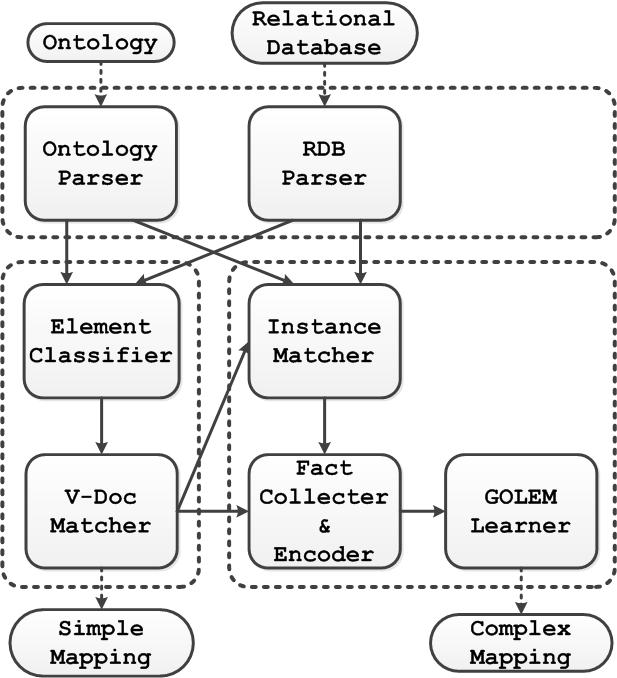
\includegraphics[height=10cm]{server}}
\caption{服务器端架构}
\label{fig:server}
\end{figure}

解析部分包含两个解析器:关系数据库解析器以及本体解析器。关系数据库解析器将用户
输入的关系数据库URL解析为关系数据库模式的元素(如表和列)及其实例(元组);本体
解析器用于将用户输入的本体URL解析为本体元素(如类和属性)及其实例(RDF数据),
解析时采用了开源的Jena API\footnote{\url{http://jena.apache.org}}。

简单映射部分包含元素分类器以及虚拟文档匹配器。元素分类器接收解析出的元素,然后
根据\ref{2:1}节中提到的分类规则将关系数据库模式和本体中的元素划分为不同的类别,
再将分类后的元素输入虚拟文档匹配器;虚拟文档匹配器在接收到不同类别的关系数据库
模式和本体元素后,采用\ref{2:2}节中的方法,对每个元素建立虚拟文档,然后计算元素
间的相似度,选取简单映射。

复杂映射部分包含实例匹配器、事实收集编码器以及GOLEM学习器。实例匹配器除了接收经
过解析的关系数据库和本体实例数据之外,还需要以已经发现的简单映射作为依据进行实例
数据的匹配;实例匹配器将经过匹配的重叠实例数据输入事实收集编码器中,事实的收集同
样需要将已经发现的简单映射作为依据,在收集到事实之后需要将其编码为谓词逻辑形式,
输入GOLEM学习器;GOLEM学习器根据输入的背景知识和正例进行学习,最终得到Horn规则
表示的复杂映射。

浏览器端界面如图\ref{fig:interface}所示,可通过web浏览器进行访问
\footnote{\url{http://ws.nju.edu.cn/smap}}。
用户可在该页面输入关系数据库模式和本体的URL以及需要发现的语义映射类型,系统完成
语义映射的发现后可将结果即时呈现在页面上。

\begin{figure}[htbp]
\centerline{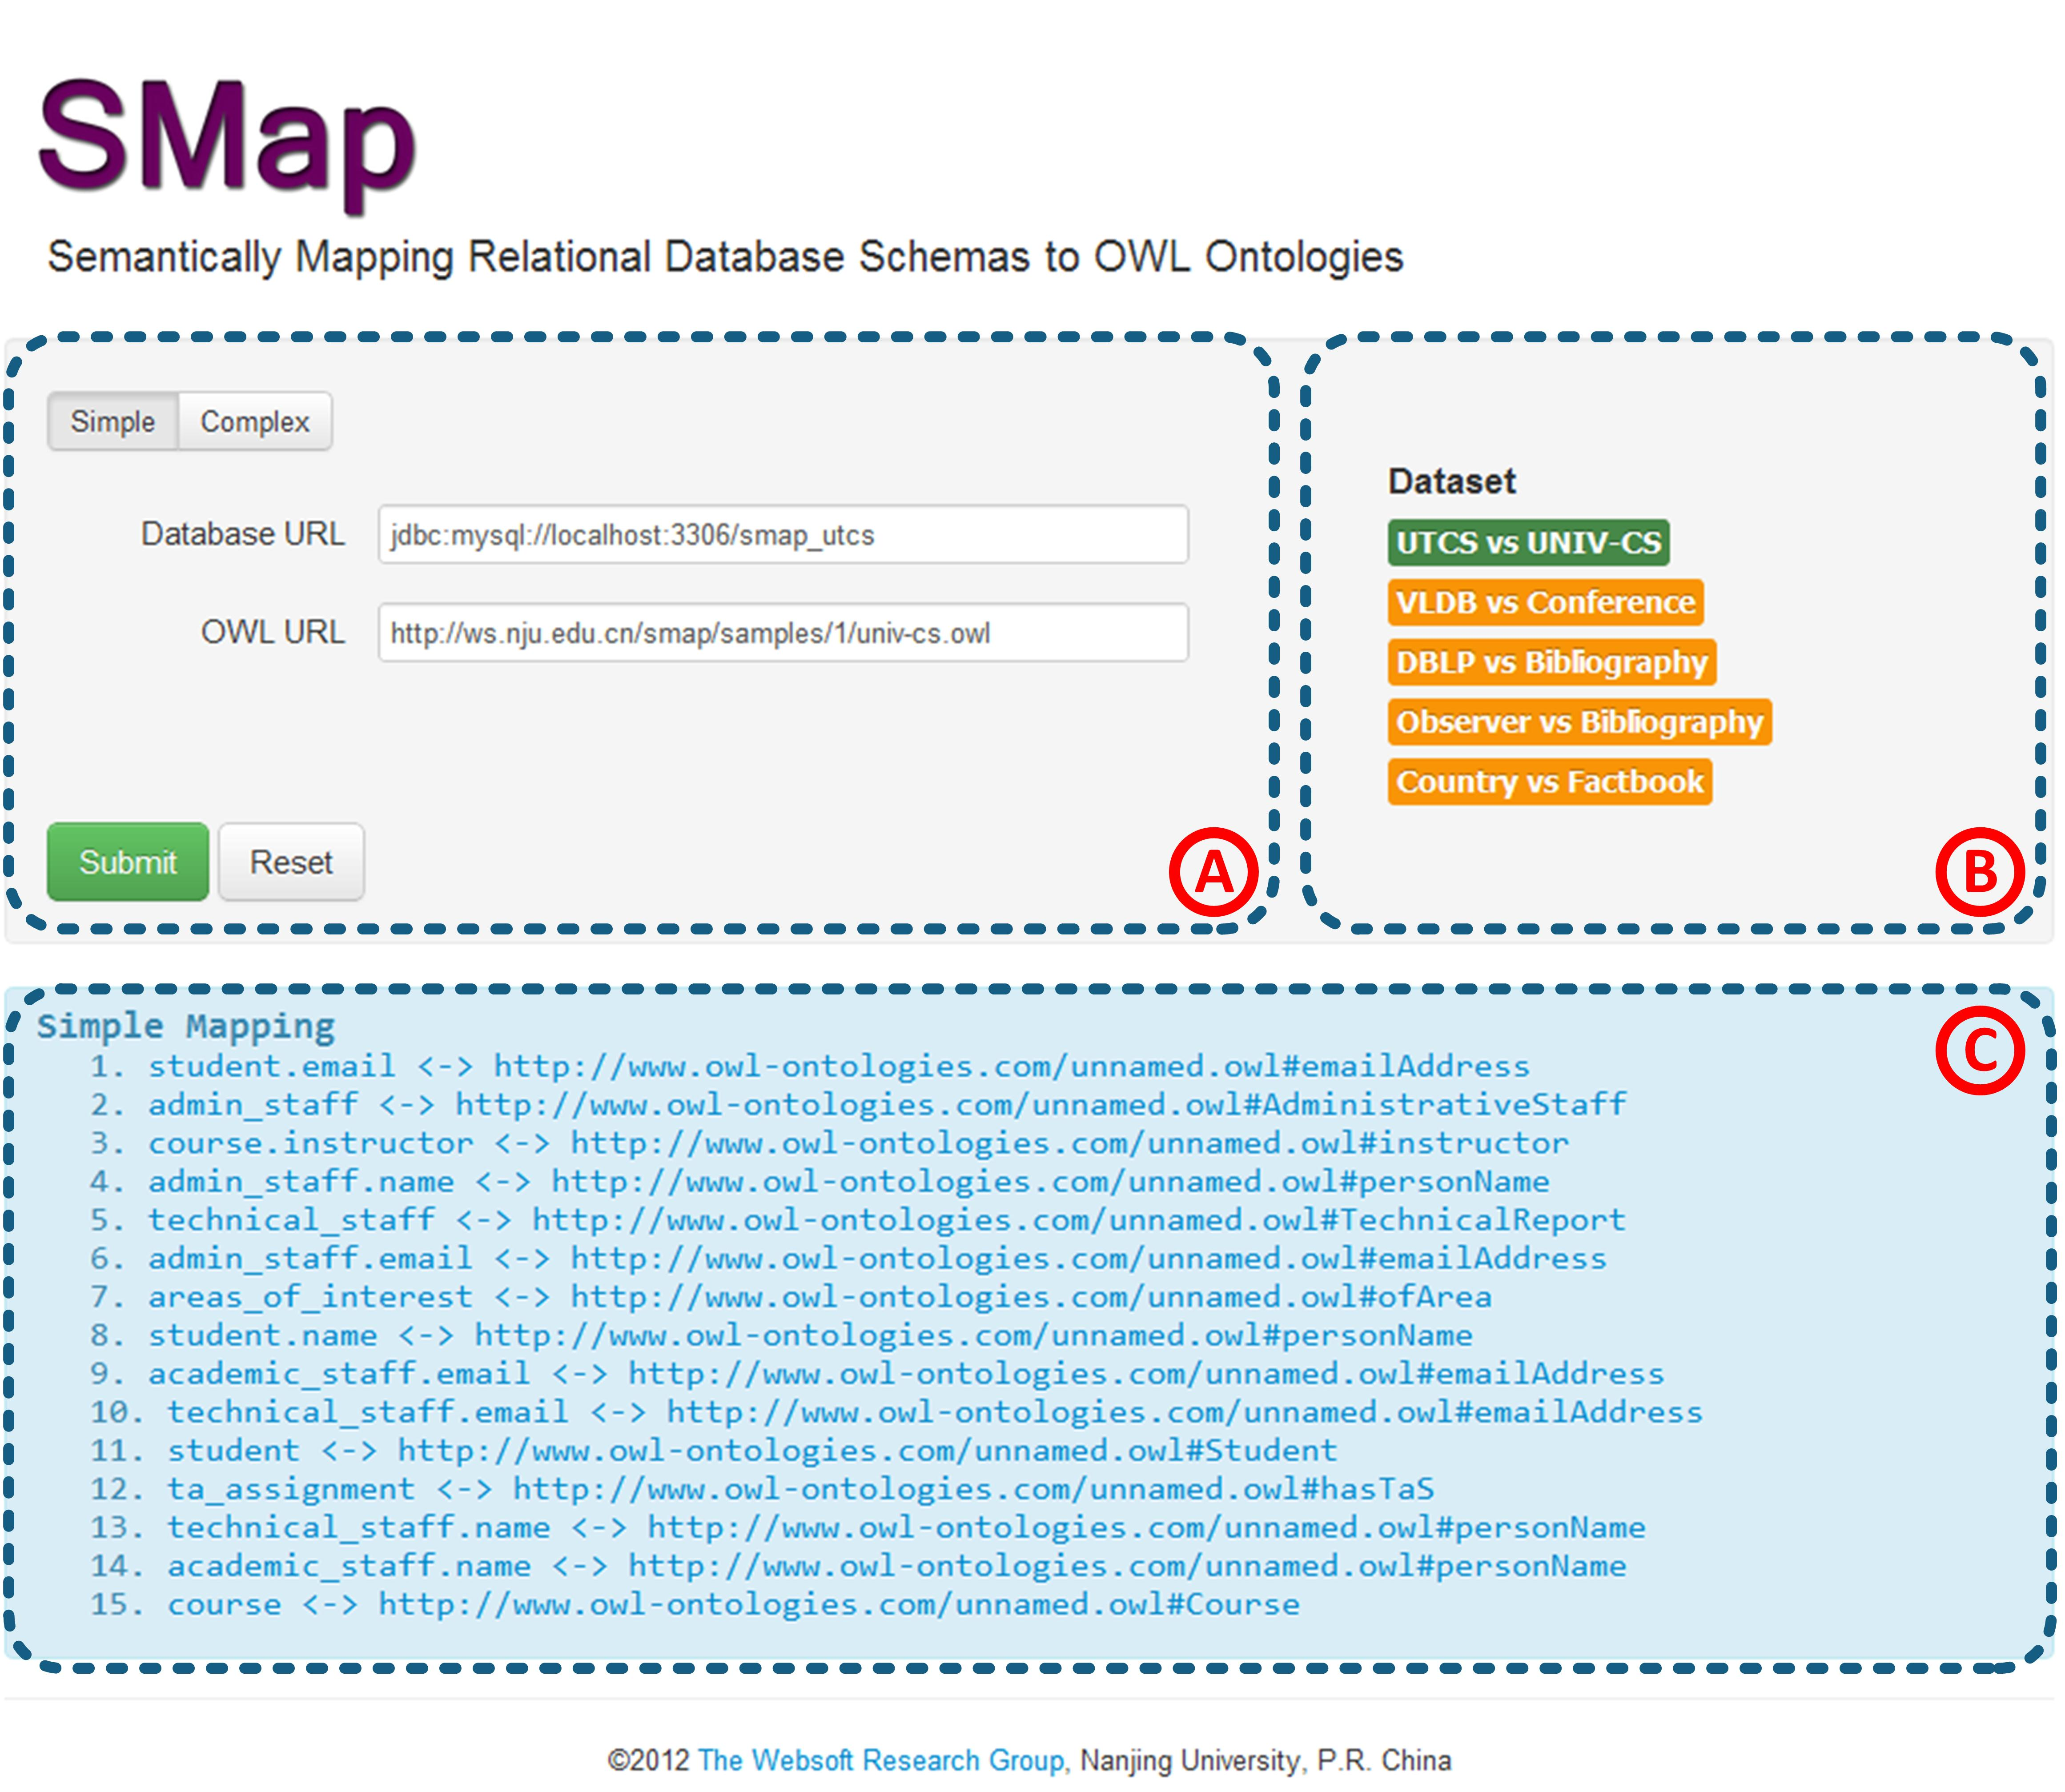
\includegraphics[width=10cm]{interface}}
\caption{浏览器端界面}
\label{fig:interface}
\end{figure}

界面主要分为3个区域,区域A为输入区,左上角的按钮用于选择需要进行发现的语义映射
类型为简单或是复杂,按钮下方的表单用于接收数据集的URL,表单下方的按钮用于提交
或重置;区域B为示例数据集区,通过点击数据集条目可将对应的示例数据集的URL自动填
入输入区中;区域C为结果区,用于呈现系统发现的语义映射。

\section{实验结果与分析}

实验选用6组测试数据集,表\ref{tab1}列出了这些测试集的统计信息。其中,前5组测试
集由MapOnto\cite{10}发布,而IBM WCC测试集由IBM公司提供。这些测试集来源于真实世
界的不同领域,并且每个测试集中的关系数据库模式与本体均相互独立。

\begin{table}[htbp]
\centering
\caption{测试数据集}
\label{tab1}
\begin{tabular}{lrrlrrrr}
\hline
\multirow{2}{*}{数据库} & \multirow{2}{*}{\#表}&\multirow{2}{*}{\#列}&
\multirow{2}{*}{本体}&\multirow{2}{*}{\#类}&\multirow{2}{*}{\#属性} &
\multicolumn{2}{c}{\#参考映射}\\
\cline{7-8}
&&&&&&简单&复杂\\
\hline
UTCS		&8	&32	&Univ-CS	&53	&35	&18	&6\\
VLDB		&9	&38	&Conference	&18	&29	&27	&4\\
DBLP		&5	&27	&Bibliography	&66	&81	&21	&4\\
Observer	&8	&115	&Bibliography	&66	&81	&72	&6\\
Country		&6	&18	&Factbook	&43	&209	&22	&5\\
IBM WCC		&279	&2187	&New WCC	&79	&276	&274	&\\
\hline
\end{tabular}
\end{table}

下面分别在简单映射发现和复杂映射学习这两个方面开展实验,并与现有工具方法进行对比
。使用精度、召回率以及F-Measure
\footnote{$\textit{F-Measure} =
\frac{2 \times \textit{召回率} \times \textit{精度}}
{\textit{召回率} + \textit{精度}}$}
(精度和召回率的线性组合)评价实验结果。评价过程中使用的参考映射由5名受过训练
的研究生手工创建。实验环境为一台拥有4GB内存的普通PC机。

\subsection{简单映射发现的实验结果与分析}
在简单映射发现方面,设计了3个对比实验来测试SMap的性能。

\theoremstyle{definition}
\newtheorem{experiment}{\heiti{实验}}
\begin{experiment}
关系数据库模式和本体中的元素是否分类对SMap的影响。这里仅使用元素自身的自然语言
描述来计算元素之间的相似度。
\end{experiment}

\begin{experiment}
\label{exp2}
是否引入相邻元素的自然语言描述对于SMap的影响,以及何种相邻元素的对结果的影响最
大。本实验中对元素进行了类型分类。相关参数设置如下:
$\alpha=0.2 \mbox{、}\beta=0.1$。在这组参数下,SMap也取得了最好的平均F-Measure。
\end{experiment}

\begin{experiment}
对比SMap与其它3个映射工具的性能。COMA++\cite{21}是目前功能最完备的映射工具之一,
它将输入模型统一转换为有向无环图的结构,因此能发现关系数据库模式与本体间的映射。
COMA++包含多种映射算法并设置了不同的映射结果组合策略。Lily\cite{22}和
AROMA\cite{23}是两个本体映射工具。本实验中先使用D2RQ将关系数据库模式转化为本体,
再分别使用它们实施本体与本体之间的映射。
\end{experiment}

图\ref{fig2}展示了是否考虑元素类型分类的对比结果。从图中可以看出,在所有测试集
中,考虑元素分类的F-Mearsure要一致优于不考虑元素分类的结果。
\begin{figure}[htbp]
\centerline{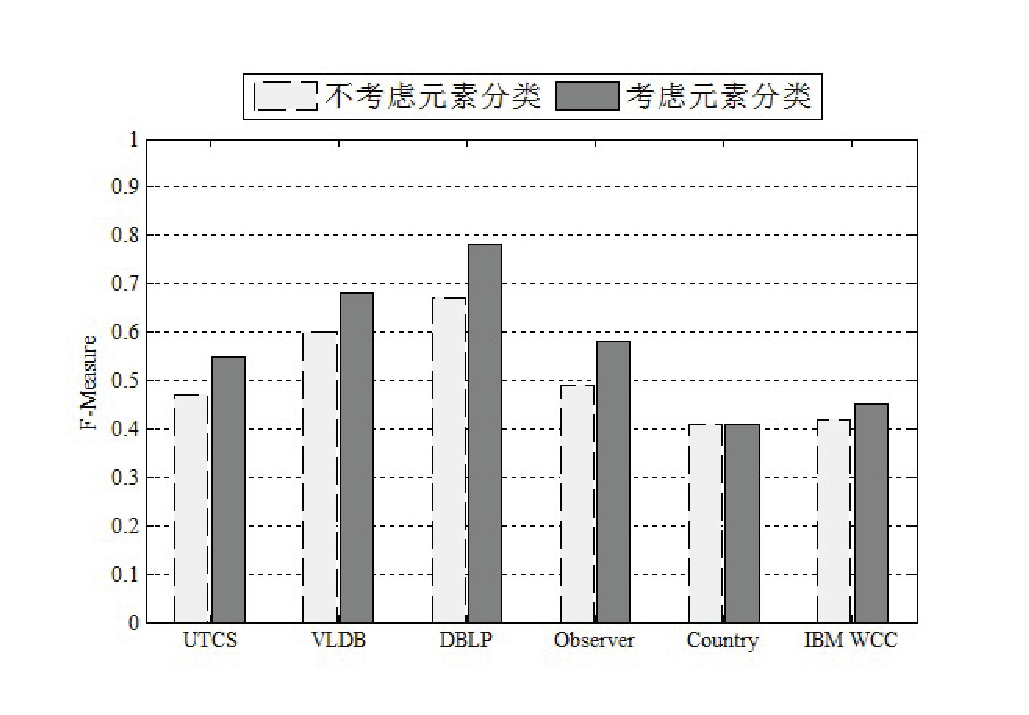
\includegraphics[width=8cm]{2}}
\caption{不考虑元素类型分类与考虑元素类型分类的F-Measure对比}
\label{fig2}
\end{figure}

实验\ref{exp2}的对比结果在图\ref{fig3}中给出。考虑相邻元素能够显著提高SMap的
F-Measure。原因在于大部分测试集中元素自身的自然语言描述较少,使用相邻元素的
描述有助于发现更多的简单映射。

\begin{figure}[htbp]
\centerline{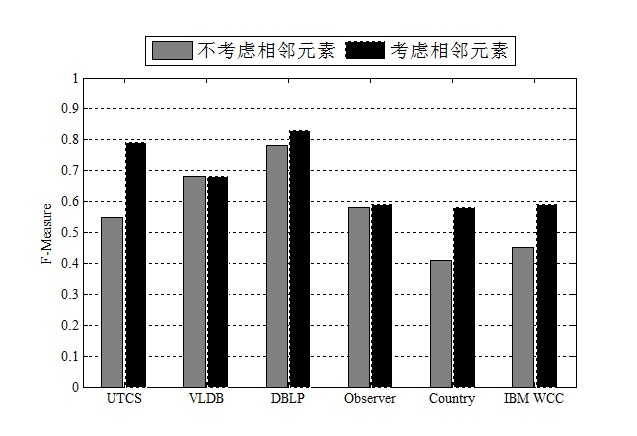
\includegraphics[width=8cm]{3}}
\caption{不考虑相邻元素和考虑相邻元素的F-Measure对比}
\label{fig3}
\end{figure}

另外,实验还对相邻元素进行了细分,发现引入关系数据库和本体属性的定义域元素对
效果提升明显,而考虑属性值域的数据类型有时反而会起到副作用,这是由于许多不同
属性都拥有相同的数据类型例如(字符型),干扰了相似度的计算。

图\ref{fig4}展示了SMap与其他3种方法在6组测试集下的平均值。精度上,SMap优于
COMA++和Lily,比AROMA差。而召回率上,SMap要明显优于其它所有工具。每个测试集的
F-Measure可参见汇总表\ref{tab2}的简单映射部分。从该表可以看出,SMap的平均
F-Measure超过其他工具20\%以上。


\begin{figure}[htbp]
\centerline{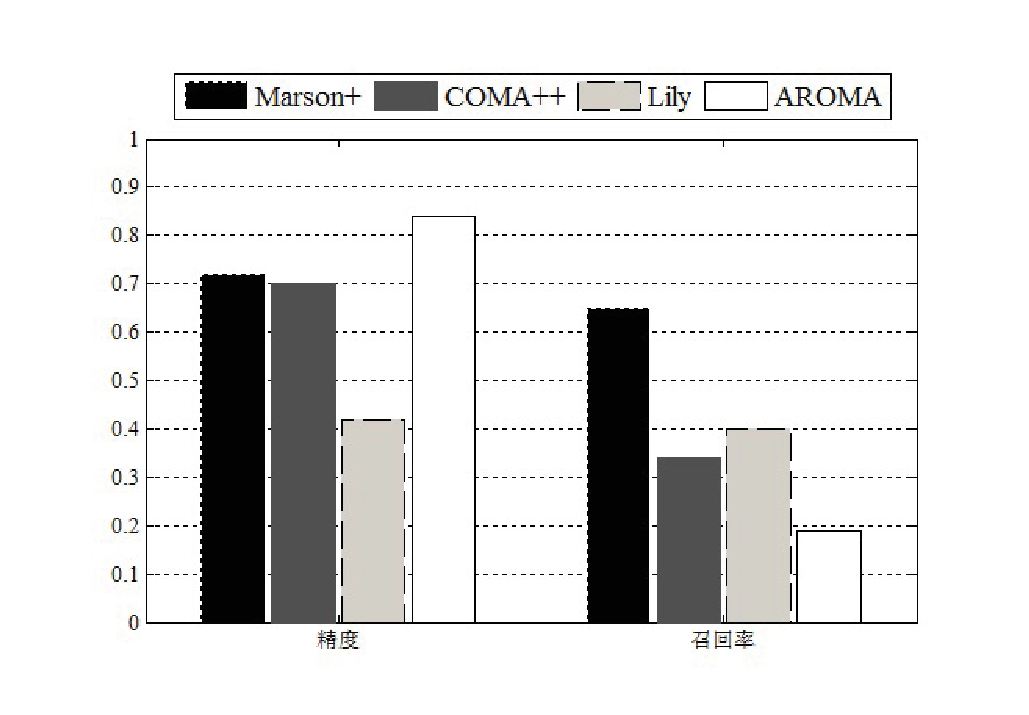
\includegraphics[width=8cm]{4}}
\caption{简单映射发现的平均精度和召回率对比}
\label{fig4}
\end{figure}


\subsection{复杂映射学习的实验结果与分析}
\begin{experiment}
比较SMap、MapOnto\cite{10}和Marson\cite{24}学习到的复杂语义映射的精度和召回率。
MapOnto需要预先构建的简单映射作为复杂映射的学习输入,故将SMap发现的简单映射输入
MapOnto。另外由于IBM WCC测试集没有公开的实例数据,因此无法在此实验中使用。
\end{experiment}

\begin{table}[htbp]
\centering
\caption{各种方法的详细实验结果汇总}
\label{tab2}
\footnotesize
\begin{tabular}{ccccccccc}
\hline
\multicolumn{2}{l}{度量指标:F-Measure} &UTCS &VLDB &DBLP &Observer &Country
&IBM WCC &平均值\\
\hline
简单映射&SMap&0.79&0.68&0.83&0.59&0.58&0.59&0.68\\
	&COMA++&解析报错&0.45&0.57&0.38&0.47&0.41&0.46\\
	&Lily&0.50&0.47&0.43&0.44&0.37&0.21&0.40\\
	&AROMA&0.29&0.43&0.25&0.10&0.43&0.32&0.30\\
\hline
复杂映射&SMap&0.92&0.89&0.86&0.67&0.73&&0.81\\
	&MapOnto&0.50&0.67&0.67&0.50&0.75&&0.62\\
	&Marson&0.50&0.40&0.40&&&&0.43\\
\hline  
\end{tabular}
\end{table}

从图\ref{fig5}的结果能够看出,3种工具的平均精度都很高,Marson更是达到了1.0。
而SMap的精度会收到实例匹配的影响。从召回率来看,SMap比其他2种工具明显要好。
通过观察其他2种工具找到的复杂映射可以发现,MapOnto主要发现了类型\ref{typ1}
的复杂映射,而Marson主要发现了类型\ref{typ3}的复杂映射。在实际数据集中,属于类
型\ref{typ1}的复杂映射最多,类型\ref{typ2}次之,类型\ref{typ3}最少,这也造成了
Marson的召回率要低于MapOnto。在运行时间方面,由于MapOnto不需要实例数据,故执行
速度较快,完成每个数据集平均耗时约0.5s。而在有200个重叠实例数据的情况下,
Marson在每个数据集上的学习耗时约1s,SMap需要约2s(仅在复杂映射学习阶段)。
\begin{figure}[htbp]
\centerline{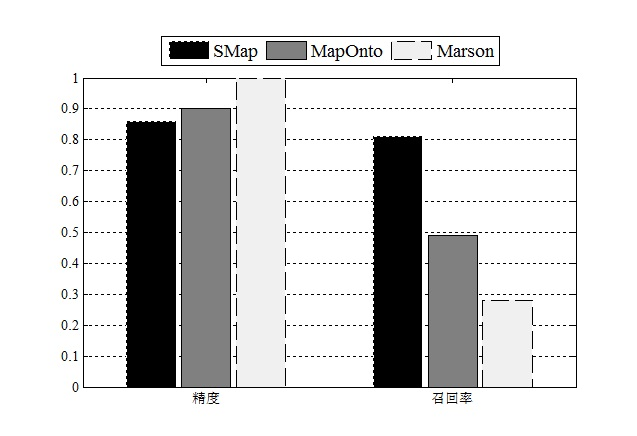
\includegraphics[width=8cm]{5}}
\caption{复杂映射学习的平均精度和召回率对比}
\label{fig5}
\end{figure}


以下为SMap学习到的一部分复杂映射:
\begin{itemize}
\item{
\textbf{\emph{DBLP}}:\emph{publisher}(\emph{name,addr}) :-
\textbf{\emph{Bibliography}}:\emph{Publisher}(\emph{A}),
\flushright{
\textbf{\emph{Bibliography}}:\emph{Agent\_name}(\emph{A,name}),
\textbf{\emph{Bibliography}}:\emph{Publisher\_Address}(\emph{A,addr}).
}}
\item{
\textbf{\emph{UTCS}}:\emph{ta\_assignment}(\emph{ctitle,sname}) :-
\textbf{\emph{Univ-CS}}:\emph{hasTaS}(\emph{B,A}),
\flushright{
\textbf{\emph{Univ-CS}}:\emph{GraduateStudent}(\emph{A}),
\textbf{\emph{Univ-CS}}:\emph{personName}(\emph{A,sname}),
\textbf{\emph{Univ-CS}}:\emph{Course}(\emph{B}),
\textbf{\emph{Univ-CS}}:\emph{courseTitle}(\emph{B,ctitle}).
}}
\item{
\textbf{\emph{VLDB}}:\emph{event}(\emph{title,\_,type,\_,\_,\_,\_}) :-
\textbf{\emph{Conference}}:\emph{Presentation}(\emph{A}),
\flushright{
\textbf{\emph{Conference}}:\emph{eventTitle}(\emph{A,title}).
}}
\end{itemize}



%\chapter{相关工作}
\label{chap05}

现有工作从多个方面研究了关系数据库模式和本体间的映射问题,例如设计映射系统的框架
、提出具体映射算法以及定义映射结果的语法语义。有关介绍请参见研究综述\cite{4,7}。

DartGrid是一个中医药领域的数据集成系统\cite{25},其中的DartMapping模块提供了一个
可视化的工具,帮助领域专家手工定义关系数据库模式与本体间的映射。OntoMat-Reverse
\cite{26}使用逆向工程规则和基于编辑距离的文本相似度计算方法,半自动地发现关系数
据库中表/列和本体中类/属性间的映射,与它类似的工作还有RONTO\cite{27}、Marson
\cite{24}等。OntoGrate框架\cite{28}首先将每个关系数据库模式转化为对应的DB本体,
然后借助记录链接和多关系数据挖掘等技术,高度自动化地发现DB本体和其他语义网本体之
间的映射。此外OntoGrate还设计了一种称为Web-PDDL的映射语言,将针对本体的查询转换
为SQL查询。类似地,StdTrip\cite{29}也是将关系数据库模式转化为本体后再实施本体映
射。MapOnto\cite{10}使用树状结构作为数据库模式和本体的中间转换模型,基于预先发现
的简单映射,在两个中间模型上迭代地传播这些映射,最终发现关系数据库模式中元素和
本体元素之间的多对多映射,并以Horn字句的形式表达。Marson则基于具有分类特性的关系
数据库列(例如性别的取值有``男''和``女''),运用决策数算法构造一类具有包含关系的
复杂映射,可以转化为基于视图的查询。

对比上述研究工作,在简单映射发现方面,本文提出了基于虚拟文档的方法,通过考察元素周
围的各种邻居元素的自然语言描述,显著提高了映射结果的效果。在复杂映射学习方面,除
MapOnto和Marson以外,其它工作还很少考虑复杂映射。MapOnto仅利用属性的定义域/值域
的兼容性构建一种句法层次上的复杂映射,Marson则是基于具有分类特性的列构造一类包含
查询,而本文运用归纳逻辑编程算法,能够从重叠实例数据中学习出多种复杂映射,覆盖面更
广。另外,数据库领域中的模式映射\cite{30}和语义网领域中的本体映射\cite{31}已经有
不少有借鉴意义的相关研究,也有工作试图将数据库模式转换为本体后再寻找映射
\cite{28,29},但是由于关系数据库模式和本体之间不存在完美的兼容关系,所以这种转换
通常是不完备的,造成了后续本体映射的精度损失。


\chapter{结束语}
\label{chap06}

本文针对关系数据库模式和OWL本体间的映射问题,提出了一种基于语义的自动化方法SMap
。首先通过元素类型分类和构建虚拟文档,发现关系数据库模式和OWL本体中元素之间的简
单映射,接下来基于这些简单映射和重叠实例数据,使用归纳逻辑编程算法学习出复杂映射
。真实数据集上的实验结果表明,在简单映射发现方面,通过逆向工程规则对元素类型进行
分类和引入邻居元素的自然语言描述,能够显著提高映射的精度和召回率,而基于归纳逻辑
编程的学习能够构建更多的复杂映射,并且学习出的复杂映射具有清晰的语义,在查询重写
等应用场景中具有重要价值。



\backmatter
\pagenumbering{Roman}
% 参考文献
\bibliographystyle{unsrt}
\bibliography{ref/reference}
\addcontentsline{toc}{chapter}{参考文献}
% 致谢
\chapter*{致\qquad 谢}
\addcontentsline{toc}{chapter}{致谢}

首先要感谢我的指导老师胡伟老师,本文从选题到定稿的每一环节都得到了他的悉心指导。在论文写作过程中,胡老师耐心地指导我进行课题的研究,还不辞辛劳地帮助我修改论文,使我的毕业论文得以顺利完成,在此致以诚挚的谢意!胡老师严谨的治学态度和认真负责的工作作风是我学习的榜样。还要感谢瞿裕忠教授,瞿教授在我进行论文写作时对我关怀有佳,提出了诸多宝贵意见,给予了我许多指导和鼓励,让我受益匪浅。

感谢实验室的各位师兄师姐,特别是师兄张航,感谢他为我在编程中提供的指导和在实验中给予的帮助。感谢08级计算机系的各位同学,感谢刘华艇 、卢俊君 、戚得信 、钱行 、钱煜 、强闰伟 、孙柯凡,能够与你们共度美好的大学时光是我最大的荣幸。

最后,感谢父母对我的养育之恩和二十余载的关怀,父母的支持是我前进的最大动力。

论文工作受国家自然科学基金(61003018);国家教育部博士点基金(20100091120041);江苏省自然科学基金(BK2011189)资助。部分工作已投稿第29届中国数据库学术会议(NDBC2012)。

\end{document}
